%% Signale.tex
%% $Id: Signale.tex 4 2005-10-10 20:51:21Z bless $
%%

Das Signal ist wie im Entwurf schon beschrieben, einer der wichtigsten Bestandteile meines Programms. 
Jedes Signal beinhaltet die Attribute Länge, Stärke, der Signaltyp sowie die Grenzen des Signaltyps.

Je nach dem in welcher Phase des Programms man sich gerade befindet, werden noch weitere Attribute gespeichert.
Das Programm besteht aus vier Phasen.

\paragraph {1. Aufnahme der Personalien}
\paragraph {2. Bestimmung der Grenzen durch Bewertung durch den Nutzer}
\paragraph {3. Ausführen des Algorithmus}
\paragraph {4. Muster Erkennung} 

Das Signal ist ein wichtiger Bestandteil meines Programm. 
Ein Signal beinhaltet die Signall{\"a}nge, die in Millisekunden gespeichert wird, und eine Signalst{\"a}rke, die in 5 St{\"a}rkestufen eingeteilt ist. 



Ich habe meinen Evolution{\"a}ren Algorithmus so angepasst, dass bei mir ein Induviduum ein Signal ist. 
Ich habe dem Benutzer das Signal mit dem Wearable abspielen lassen und im Anschluss Fragen beantworten lassen. 
Er sollte bewerten wie gut er das Signal erkannt hat. Die Bewertung vom Benutzer war entscheidend um nach der kompletten Bewertung der Population 









% -----------------------------------------------------------------------

\paragraph {1. Aufnahme der Personalien}

\begin{figure}[htbp] 
	\centering
	\begin{minipage}[t]{0.45\textwidth}
		\includegraphics[width=\textwidth]{pics/gui/{AngabenZurPerson1}.png}
	\end{minipage}
	\begin{minipage}[t]{0.45\textwidth}
		\includegraphics[width=\textwidth]{pics/gui/{AngabenZurPerson2}.png}
	\end{minipage}
	\caption{}
	\label{fig:Bild10}
\end{figure}

Um in der Evaluierung mögliche Erkentnisse zwischen bestimmten Benutzergruppen herausfinden zu können, hat man dem Benutzer Eine Reihe von Fragen gestellt, die im Bild XXXX zu sehen sind.
Diese Daten wurden anonymisiert gespeichert. 
\paragraph {2. Bestimmung der Grenzen durch Bewertung durch den Nutzer}

\begin{figure}
	\centering
    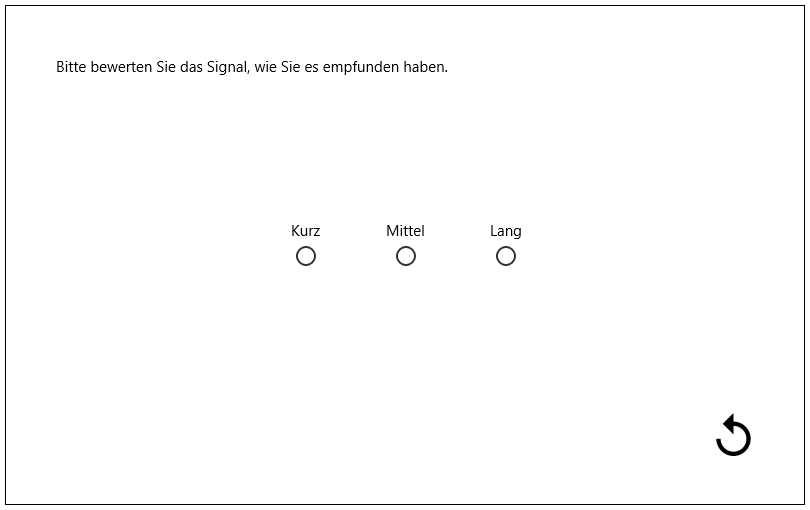
\includegraphics[width=\textwidth]{pics/gui/GrenzenBestimmen.png}
    \caption{Settings on the apple watch}
    \label{fig:applewatch}
\end{figure}

\paragraph {3. Ausführen des Algorithmus}

\begin{figure}[htbp] 
	\centering
	\begin{minipage}[t]{0.45\textwidth}
		\includegraphics[width=\textwidth]{pics/gui/{Algorithmus1}.png}
	\end{minipage}
	\begin{minipage}[t]{0.45\textwidth}
		\includegraphics[width=\textwidth]{pics/gui/{Algorithmus2Emotion}.png}
	\end{minipage}
	\caption{}
	\label{fig:Bild10}
\end{figure}

\paragraph {4. Muster Erkennung} 

MUSTER BILD

